\documentclass[]{article}
\makeatletter
\usepackage{lmodern}
\usepackage{comment}
\excludecomment{Answ}
\newcounter{ItemCounter}
\usepackage{listings}
\usepackage{color} %red, green, blue, yellow, cyan, magenta, black, white
\definecolor{mygreen}{RGB}{28,172,0} % color values Red, Green, Blue
\definecolor{mylilas}{RGB}{170,55,241}
\renewcommand\paragraph{\@startsection{paragraph}{4}{\z@}%
            {-2.5ex\@plus -1ex \@minus -.25ex}%
            {1.25ex \@plus .25ex}%
            {\normalfont\normalsize\bfseries}}
\makeatother
\newcommand{\myvec}[1]{\ensuremath{\begin{pmatrix}#1\end{pmatrix}}}
\usepackage{gensymb}
\setcounter{secnumdepth}{4}
\usepackage{amsmath}
%\usepackage{mathtools}
\usepackage{graphicx}
\usepackage{slashed}
\usepackage{lineno}
\usepackage{latexsym}
\usepackage{subfigure}
\usepackage{amssymb}
\newtheorem{thm}{Theorem}[section]
\newtheorem{cor}[thm]{Corollary}
\newtheorem{lem}[thm]{Lemma}
\usepackage[numbers,sort]{natbib}
\usepackage{enumerate}
\newcommand{\bb}{\begin{equation}}
\newcommand{\ee}{\end{equation}}
\newtheorem{defin}{Definition}
\usepackage{multirow}
\usepackage{ctable}
\usepackage{bm}
\usepackage{enumerate}
\newcommand{\D}[2]{\frac{\partial #1}{\partial #2}}
\newcommand{\DD}[2]{\frac{\partial^2 #1}{\partial #2^2}}
\newcommand{\rd}{\text{ d}}
\usepackage{framed}
\newcommand{\see}[1]{(see Figure \ref{#1})}
\newcommand{\fig}[1]{Figure \ref{#1}}
\newcommand{\figs}[2]{figures \ref{#1} and \ref{#2}}
\newcommand{\sect}[1]{Section \ref{#1}}
\newcommand{\app}[1]{Appendix \ref{#1}}
\newcommand{\chap}[1]{Chapter \ref{#1}}
\newcommand{\eqn}[1]{equation \eqref{#1}}
\newcommand{\eqns}[2]{equations \eqref{#1} and \eqref{#2}}
\newcommand{\eqnto}[2]{equations \eqref{#1}-\eqref{#2}}
%\usepackage{authblk}
\usepackage{url}
\usepackage{soul}
\newcommand{\eg}{\emph{e.g.} }
\newcommand{\bn}{\bm{n}}
\newcommand{\bu}{\bm{u}}
\newcommand{\ie}{\emph{i.e.} }
\newcommand{\Chapter}[1]{\chapter{#1}\label{#1}}
\newcommand{\Section}[1]{\section{#1}\label{#1}}
\newcommand{\Subsection}[1]{\subsection{#1}\label{#1}}
\newcommand{\Subsubsection}[1]{\subsubsection{#1}\label{#1}}
\newcommand{\Appendix}[1]{\appendix{#1}\label{#1}}
\usepackage[margin=1.5cm,centering]{geometry}
\usepackage[geometry]{ifsym}
\makeatletter
\newcommand\restr[2]{{% we make the whole thing an ordinary symbol
  \left.\kern-\nulldelimiterspace % automatically resize the bar with \right
  #1 % the function
  \vphantom{\big|} % pretend it's a little taller at normal size
  \right|_{#2} % this is the delimiter
  }}
\def\url@leostyle{%
  \@ifundefined{selectfont}{\def\UrlFont{\sf}}{\def\UrlFont{\small\ttfamily}}}
\makeatother
\urlstyle{leo}
\usepackage{multirow}
\usepackage{blkarray}
\usepackage{soul}
\usepackage{framed}
\usepackage{color}
\usepackage{setspace}
\newcommand{\ttttp}{.24\textwidth}
\newcommand{\tttp}{.32\textwidth}
\newcommand{\ttp}{.45\textwidth}
\newcommand{\tbo}{.6\textwidth}
 \usepackage[T1]{fontenc}
\usepackage[utf8]{inputenc}
\usepackage{authblk}
 \renewcommand{\l}{\left(}
\renewcommand{\r}{\right)}
%\begin{figure}[h!!!tb]
%\centering
%\subfigure[\label{Godzilla}]{\includegraphics[height=0.35\textwidth]{./Pictures/Godzilla_final_bw.png}}
%\subfigure[\label{Jaeger}]{\includegraphics[height=0.35\textwidth]{./Pictures/Jaeger_finish_bw.png}}
%\caption{\label{Monsters} The two types of monster we are going to consider are: (a) the naturally occurring Kaijus and (b) the man-made Jaegers.}
%\end{figure}


\begin{document}

\lstset{language=Matlab,%
    %basicstyle=\color{red},
    breaklines=true,%
    morekeywords={matlab2tikz},
    keywordstyle=\color{blue},%
    morekeywords=[2]{1}, keywordstyle=[2]{\color{black}},
    identifierstyle=\color{black},%
    stringstyle=\color{mylilas},
    commentstyle=\color{mygreen},%
    showstringspaces=false,%without this there will be a symbol in the places where there is a space
    numbers=left,%
    numberstyle={\tiny \color{black}},% size of the numbers
    numbersep=9pt, % this defines how far the numbers are from the text
    emph=[1]{for,end,break},emphstyle=[1]\color{red}, %some words to emphasise
    %emph=[2]{word1,word2}, emphstyle=[2]{style},    
}


\title{Problem sheet 2}
\author{Thomas E. Woolley\\Last edited on:}
\maketitle
\section{Time derivatives of polar coordinates}\label{Polar_derivatives}
In this question we are going to be converting between Cartesian and polar coordinates. Moreover, we will be using the transformation relationships to take time derivatives of the polar coordinates. Critically, we will be using symbols, $r$, $\bm{r}$ and $\hat{\bm{r}}$. This may seem confusing (because it is), however, these are standard names for the variables we are going to consider. Thus, my advice to you is to be careful over which variable you mean. Note that, although this question seems long, it is split up into a number of small chunks to help you through, thus, each question only requires a small answer.

Consider \fig{Polars}, where we see a point $(x,y)$, which is a distance $r$ away from the origin along an angle $\theta$ away from the horizontal. Equally, define $\bm{i}$ and $\bm{j}$ to be the standard normalised Cartesian vectors,
\bb
\myvec{1\\0}, \quad\myvec{0\\1}
\ee
respectively. Further, let $\hat{\bm{r}}$ and $\hat{\bm{\theta}}$ be the normalised polar coordinates along the radial and angular directions as shown.
\begin{figure}[h!!!tb]
\centering
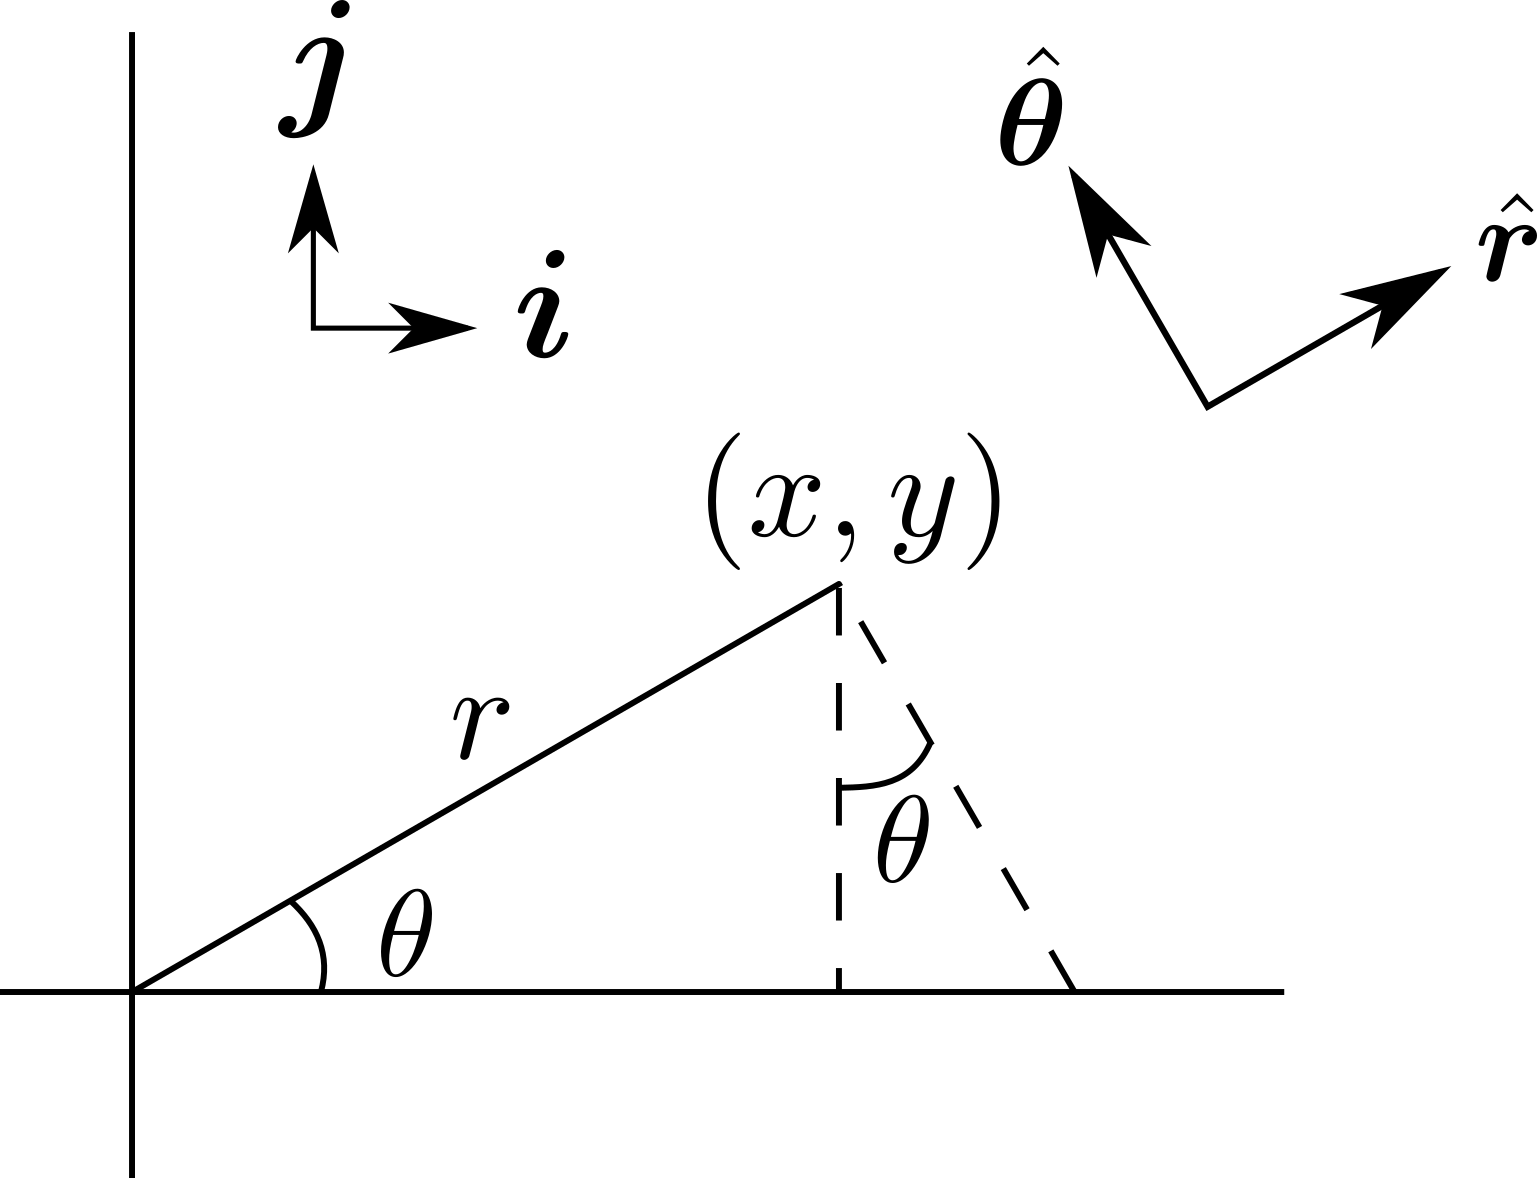
\includegraphics[width=\ttp]{../../Pictures/Polars.png}
\caption{\label{Polars} Cartesian and polar coordinates.}
\end{figure}
\begin{enumerate}
\item \label{1} From \fig{Polars} we can derive that relationship that
\bb
\hat{\bm{\theta}}=\myvec{-\sin(\theta)\\ \cos(\theta)}.
\ee
What is the equivalent relationship for $\hat{\bm{r}}$.
\item \label{2} Rewrite the general coordinate vector
\bb
\bm{r}=\myvec{x\\y}
\ee
in terms $r$, $\theta$, $\cos$ and $\sin$.
\item \label{3} Using questions \ref{1} and \ref{2} show that we can rewrite the coordinate vector $\bm{r}$ as
\bb
\bm{r}=r\hat{\bm{r}}.
\ee
\item \label{4} Using question \ref{1} show that
\bb
\dot{\hat{\bm{r}}}=\myvec{-\sin(\theta)\\\cos(\theta)}\dot{\theta}.
\ee
\item \label{5} Find a similar results for $\dot{\hat{\bm{\theta}}}$.
\item \label{6} Rewrite the results of questions \ref{4} and \ref{5} to give $\dot{\hat{\bm{r}}}$ and $\dot{\hat{\bm{\theta}}}$ in terms of $\hat{\bm{r}}$ and $\hat{\bm{\theta}}$.
\item \label{7} Combine questions \ref{3} and \ref{6} to show that
\bb
\dot{\bm{r}}=\dot{r}\hat{\bm{r}}+r\dot{\theta}\hat{\bm{\theta}}.
\ee
\item \label{8} Use question \ref{6} again to take a second derivative of the position vector to show that
\bb
\ddot{\bm{r}}=\l\ddot{r}-r\dot{\theta}^2\r\hat{\bm{r}}+\l 2\dot{r}\dot{\theta}+r\ddot{\theta}\r\hat{\bm{\theta}}.
\ee
\item \label{9} Assume now that the position is evolving due to an applied force, $\bm{F}$, but there is no component of force along the $\hat{\bm{\theta}}$ direction, \ie $\bm{F}=F\hat{\bm{r}}$. Use Newton's Second Law of Motion to show that
\bb
F=m\l\ddot{r}-r\dot{\theta}^2\r,
\ee
where $m$ is the mass of the object the force is acting on and
\bb
r^2\dot{\theta}=\textrm{constant}.\label{Kepler}
\ee
\end{enumerate}
Having finished question \ref{9} you will have proven Kepler's Second Law of Planetary Motion. Namely, if we consider a planet orbiting a sun then a line segment joining the centres of the planet and the Sun sweeps out equal areas during equal intervals of time. This comes from the above result because the force acting on an orbiting planet will be gravitation, which acts along a line connecting the centres of the planets, \ie there is no angular component to the force. Thus, \eqn{Kepler} holds and $r^2\dot{\theta}$ has the interpretation of being the area swept out by the line connecting the two bodies, which is derived to be constant.
\begin{figure}[h!!!tb]
\centering
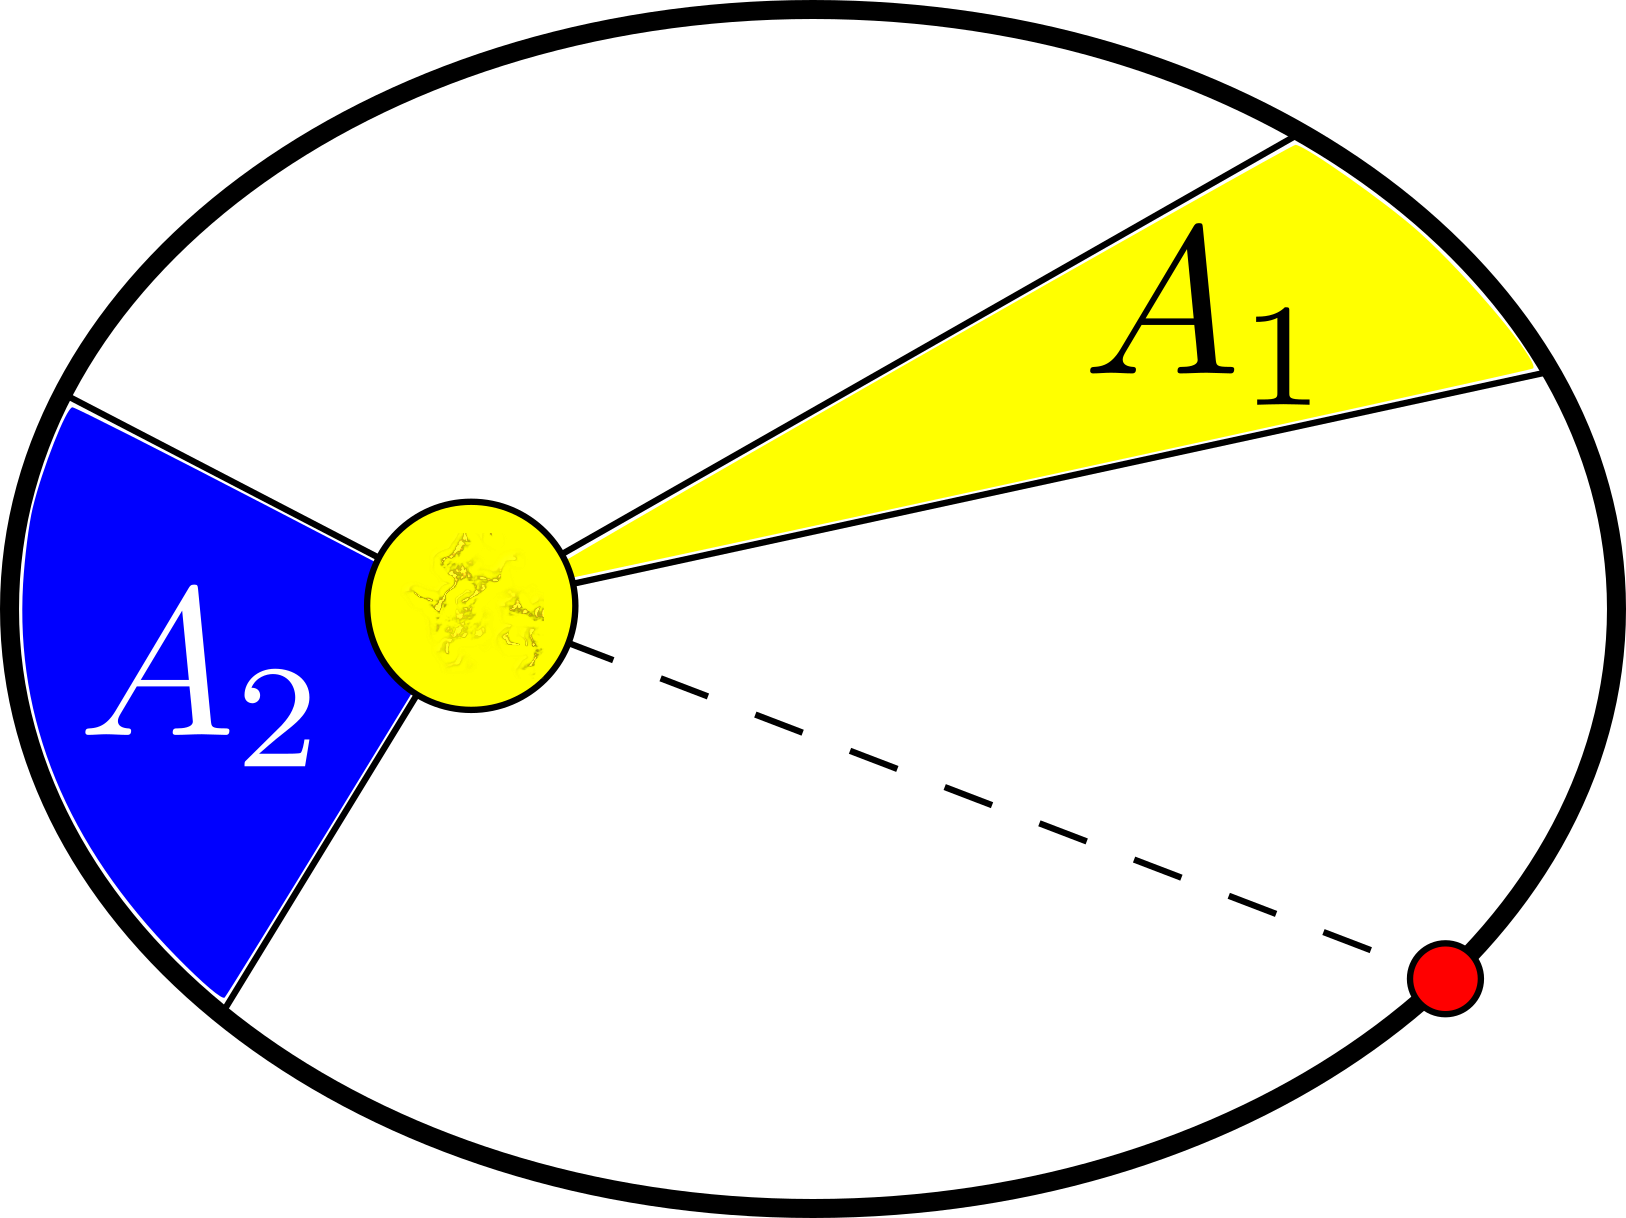
\includegraphics[width=\ttp]{../../Pictures/Kepler.png}
\caption{\label{Kepler_law} Illustrating Kepler's Second Law of Planetary motion. Suppose $A_1$ and $A_2$ are areas swept out by the line connecting the red planet to the yellow sun in the same amount of time. Then \eqn{Kepler} proves $A_1=A_2$.}
\end{figure}
\begin{Answ}
\subsection{Answer}
\subsubsection{}
\bb
\hat{\bm{r}}=\myvec{\cos(\theta)\\ \sin(\theta)}, \quad \hat{\bm{\theta}}=\myvec{-\sin(\theta)\\ \cos(\theta)}.
\ee
\subsubsection{}
\bb
\bm{r}=\myvec{r\cos(\theta)\\r\sin(\theta)}.
\ee
\subsubsection{}
\bb
\bm{r}=\myvec{r\cos(\theta)\\r\sin(\theta)}=r\myvec{\cos(\theta)\\\sin(\theta)}=r\hat{\bm{r}}.
\ee
\subsubsection{}
Taking derivatives of each component separately and remembering that by chain rule $\rd f(u)/\rd t=f'(u)\rd u/\rd t$ we derive
\bb
\dot{\hat{\bm{r}}}=\myvec{-\sin(\theta)\dot{\theta}\\\cos(\theta)\dot{\theta}}.\label{rdot}
\ee
\subsubsection{}
\bb
\dot{\hat{\bm{\theta}}}=\myvec{-\cos(\theta)\dot{\theta}\\-\sin(\theta)\dot{\theta}}.\label{thetadot}
\ee
\subsubsection{}
Comparing the vectors forms in \eqns{rdot}{thetadot}
\bb
\dot{\hat{\bm{\theta}}}=-\hat{\bm{r}}\dot{\theta},\quad
\dot{\hat{\bm{r}}}=\hat{\bm{\theta}}\dot{\theta}.
\ee
\subsubsection{}
\bb
\dot{\bm{r}}=\frac{\rd \l r\hat{\bm{r}} \r}{\rd t}=\dot{r}\hat{\bm{r}}+r\dot{\hat{\bm{r}}}=\dot{r}\hat{\bm{r}}+r\dot{\theta}\hat{\bm{\theta}}.
\ee
\subsubsection{}
\bb
\ddot{\bm{r}}=\frac{\rd \l \dot{r}\hat{\bm{r}}+r\dot{\theta}\hat{\bm{\theta}} \r}{\rd t}=\ddot{r}\hat{\bm{r}}+\dot{r}\dot{\hat{\bm{r}}}+\dot{r}\dot{\theta}\hat{\bm{\theta}}+r\ddot{\theta}\hat{\bm{\theta}}+r\dot{\theta}\dot{\hat{\bm{\theta}}}=\l \ddot{r}-r\dot{\theta}^2\r\hat{\bm{r}}+\l 2\dot{r}\dot{\theta}+r\ddot{\theta}\r\hat{\bm{\theta}}.
\ee
\subsubsection{}
If there is no force along the angular direction then by Newton's Second Law of Motion (Force=Mass$\times$Acceleration)
\bb
2\dot{r}\dot{\theta}+r\ddot{\theta}=0.\label{FMA}
\ee
Equation \eqref{FMA} can be rewritten as a full derivative
\bb
\frac{1}{r}\frac{\rd}{\rd t}\l r^2\dot{\theta}\r=0.
\ee
Integrating provides the result
\bb
r^2\dot{\theta}=\textrm{constant}.
\ee
\end{Answ}
\section{Two body problem}
Consider two planets with the same mass, $m$, and positions $\bm{r}_1(t)$ and $\bm{r}_2(t)$, respectively. Let the initial positions be $\bm{r}_1(0)=\bm{r}_{10}$ and $\bm{r}_2(0)=\bm{r}_{20}$ and let the initial velocities be $\dot{\bm{r}}_1(0)=\bm{v}_{10}$ and $\dot{\bm{r}}_2(0)=\bm{v}_{20}$.
\begin{figure}[h!!!tb]
\centering
\subfigure[\label{TBP_1}]{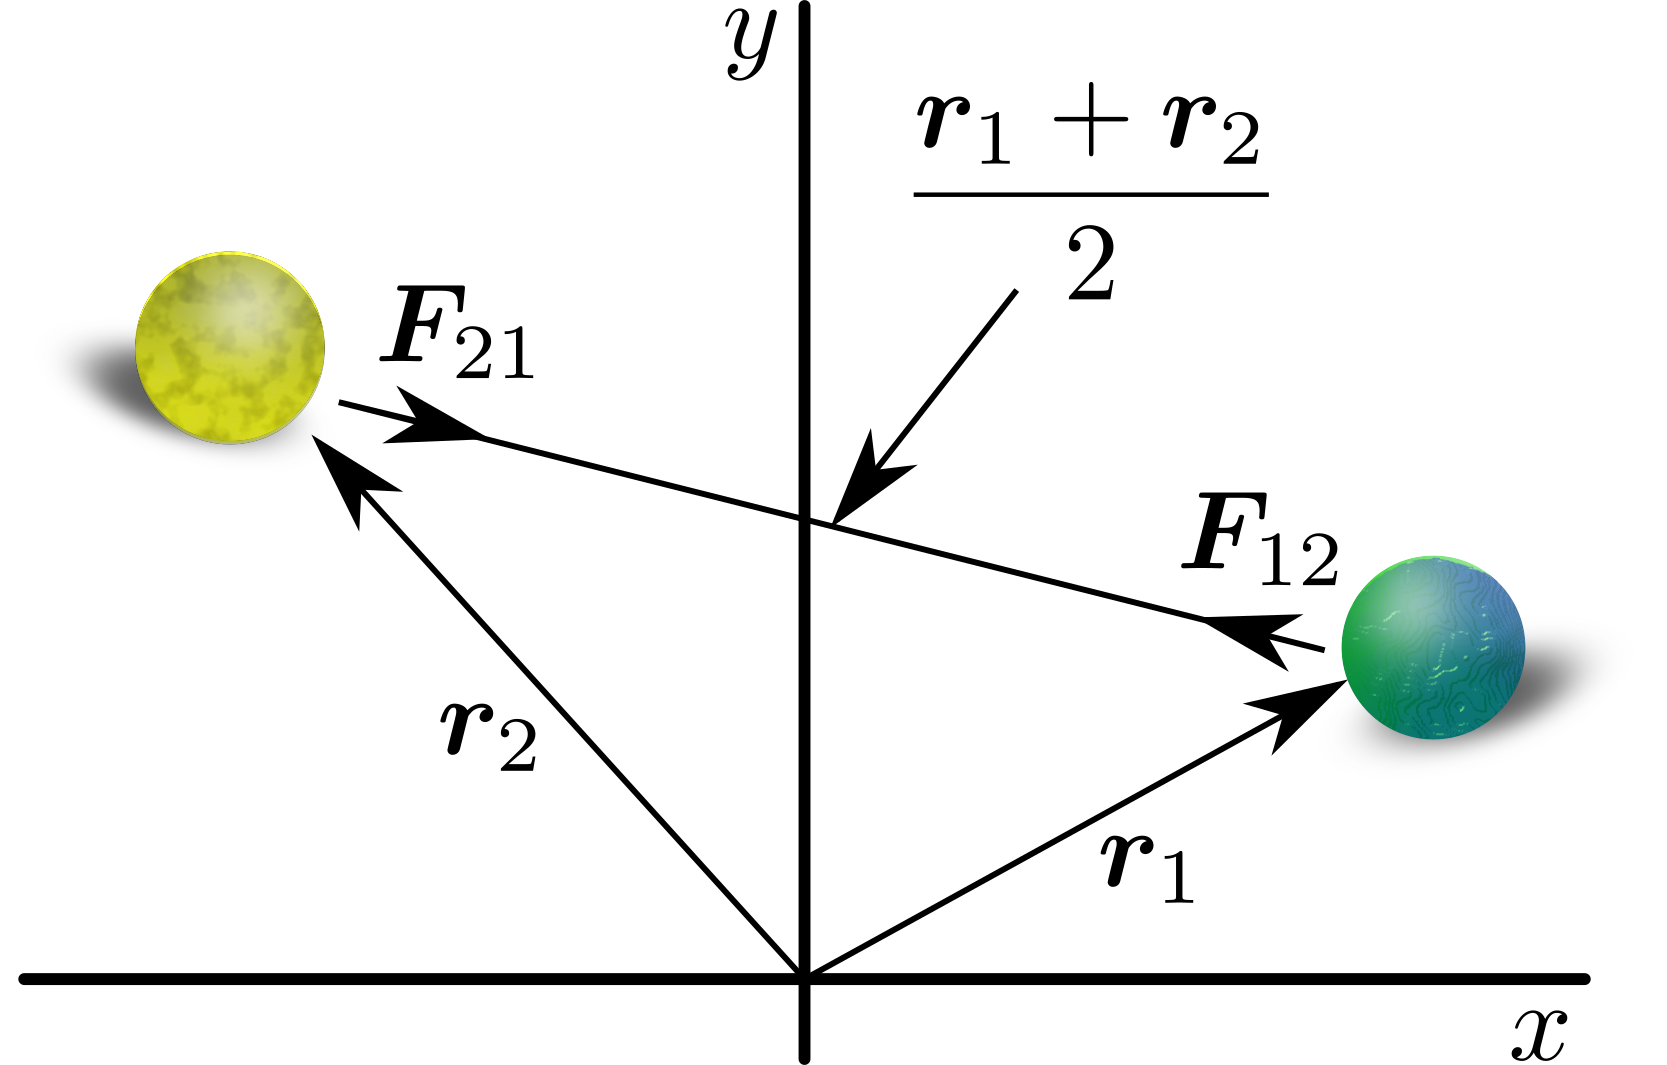
\includegraphics[width=\ttp]{../../Pictures/Two_body_problem.png}}
\subfigure[\label{TBP_2}]{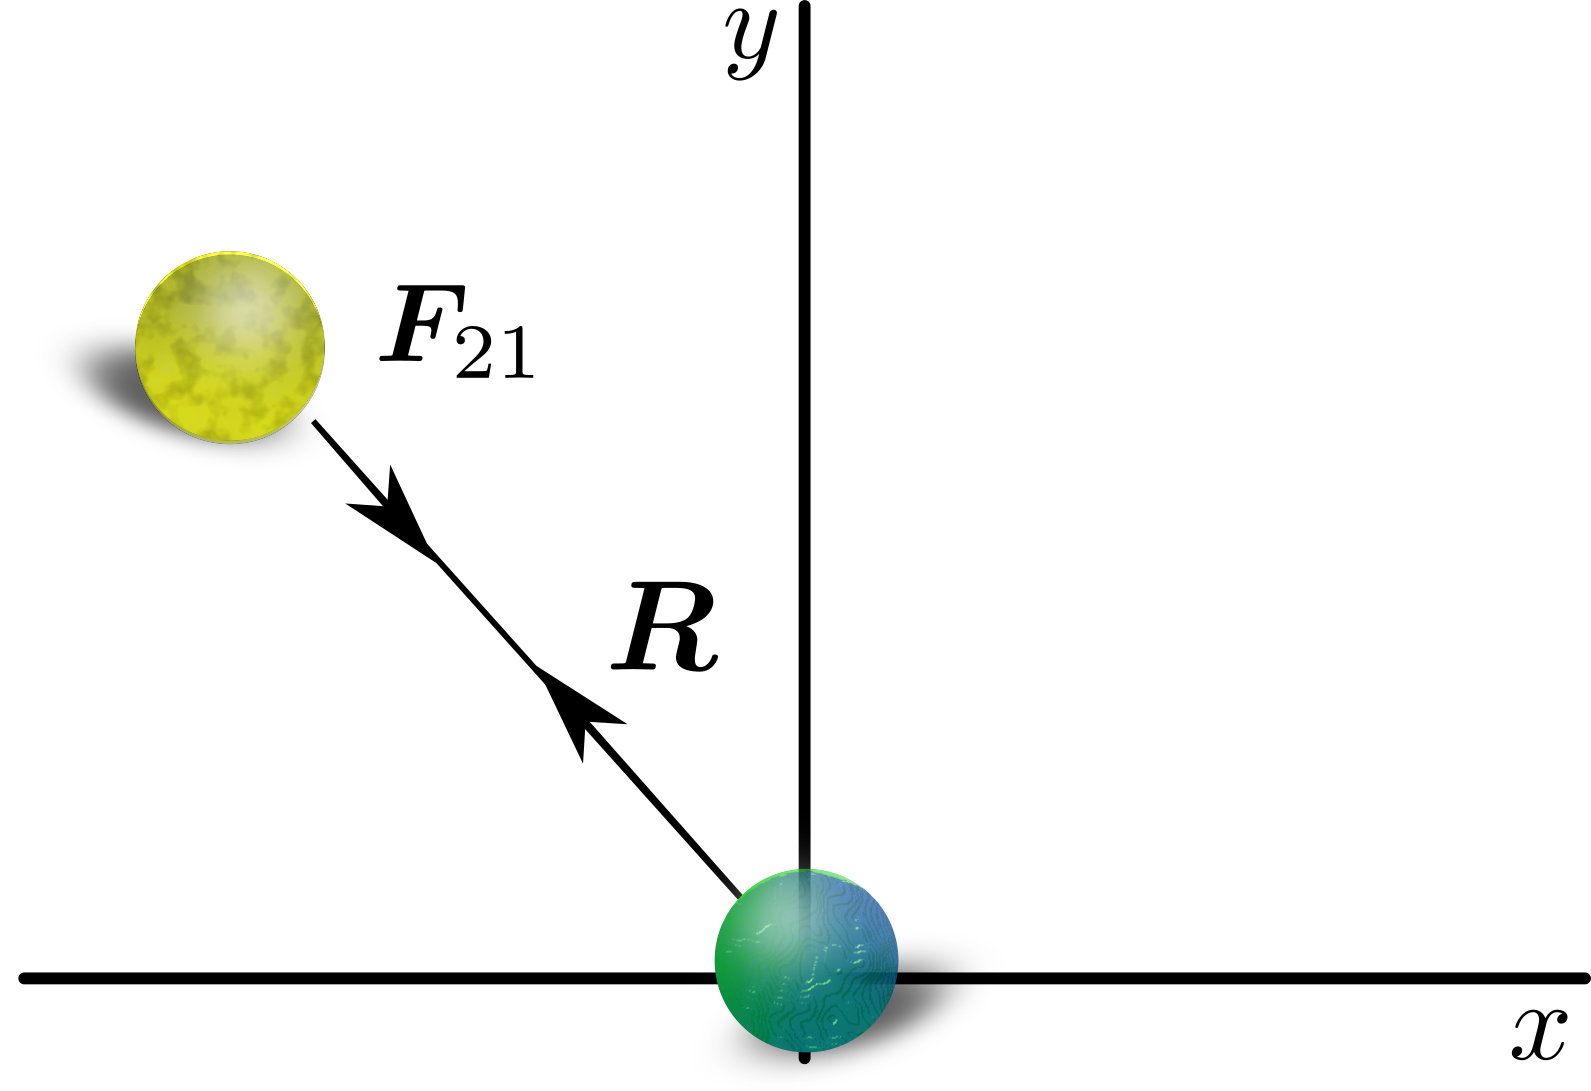
\includegraphics[width=\ttp]{../../Pictures/Two_body_problem_new_origin.png}}
\caption{\label{Two_body_problem} (a) Positions and forces in the two body problem. The position $(\bm{r}_1+\bm{r}_2)/2$ is the centre of mass of the two body system. (b) Redefining the system so that planet 1 is the origin.}
\end{figure}
\begin{enumerate}
\item Using Newton's Law of Gravitation what are the forces $\bm{F}_{12}$ and $\bm{F}_{21}$.
\item \label{Planet_N2L}Using Newton's Second Law of Motion, write down two governing equations for the positions of the two planets in terms of the forces derived in part 1 and the accelerations, $\ddot{\bm{r}}_1$ and $\ddot{\bm{r}}_2$. Deduce that
\bb
\ddot{\bm{r}}_1+\ddot{\bm{r}}_2=0.
\ee
By proving this result and considering \fig{TBP_1} we see that the the  centre  of  mass  of  the  two-body  system  exhibits  no acceleration. Thus, as the two planets orbit each other they can travel through space, but their movement must be consistent with the fact that their centre of mass is stationary, or moving at a constant speed.
\setcounter{ItemCounter}{\value{enumi}}
\end{enumerate}


%\item Use part \ref{8} from question \ref{Polar_derivatives} to separate the two equations  derived in \ref{Planet_N2L} into the coordinate components $(r_1,\theta_1)$ and $(r_2,\theta_2)$.
%
%\bb
%\l \ddot{r}_1-r\dot{\theta}_1^2\r\hat{\bm{r}}+\l 2\dot{r}_1\dot{\theta}_1+r_1\ddot{\theta}_1\r\hat{\bm{\theta}}=-\frac{Gm}{|r_1-r_2|^2}\hat{\bm{r}}_{12}.
%\ee
%
%
%Hint: Define $\hat{\bm{r}}$ and $\hat{\bm{\theta}}$ to be the radial and angular unit variables as in question 1 then $\bm{r}_1=r_1\hat{\bm{r}}$ and $\bm{r}_2=r_2\hat{\bm{r}}$ such that $|\bm{r}_1-\bm{r}_2|=|\bm{r}_1-\bm{r}_2|=|r_1-r_2|$.
%
%
%\item Since the gravitational force between two bodies does not have a force component along the angular direction we should be able to simplify the equations to
%\bb
%\ddot{r}_1-r_1\dot{\theta}_1^2=-G\frac{m}{|r_1-r_2 |^2},\quad \ddot{r}_2-r_2\dot{\theta}_2^2=G\frac{m}{|r_1-r_2|^2},
%\ee
%\bb
%r_1^2\dot{\theta_1}=c_1, \quad r_2^2\dot{\theta_2}=c_2.
%\ee
%where $c_1$ and $c_2$ are constants.
\begin{Answ}
\subsection{Answers}
\subsubsection{}
\bb
\bm{F}_{21}=-G\frac{m^2}{|\bm{r}_2-\bm{r}_1 |^3}\l \bm{r}_2-\bm{r}_1\r,\quad \bm{F}_{12}=-G\frac{m^2}{|\bm{r}_1-\bm{r}_2 |^3}\l \bm{r}_1-\bm{r}_2\r.
\ee
\subsubsection{}
\bb
m\ddot{\bm{r}}_1=-G\frac{m^2}{|\bm{r}_1-\bm{r}_2 |^3}\l \bm{r}_1-\bm{r}_2\r,\quad m\ddot{\bm{r}}_2=-G\frac{m^2}{|\bm{r}_2-\bm{r}_1 |^3}\l \bm{r}_2-\bm{r}_1\r.
\ee
By adding the two equations together we indeed discover that the sum of the accelerations is zero, as required.
\end{Answ}
\section{Two body problem continued}\label{Two body problem continued}
Instead of considering the two positions separately, we redefine the origin to be planet 1 and consider the motion of planet 2 relative to planet 1 \see{TBP_2}. Thus, we let $\bm{R}=\bm{r}_2-\bm{r}_1$ be the new position vector, where $R=|r_2-r_1|$ is the distance between the two planets and the position vector makes an angle $\Theta$ against the positive horizontal. From this define $\hat{\bm{R}}$ and $\hat{\bm{\Theta}}$ to be the new unit vectors in the radial and angular directions. By Newton's Second Law of Motion (see question \ref{Polar_derivatives}) the equation governing the system is
\bb
\l \ddot{R}-R\dot{\Theta}^2\r\hat{\bm{R}}+\l 2\dot{R}\dot{\Theta}+R\ddot{\Theta}\r\hat{\bm{\Theta}}=-\frac{Gm}{R^2}\hat{\bm{R}}
\ee
or, from question \ref{Polar_derivatives},
\bb
\ddot{R}-R\dot{\Theta}^2=-\frac{Gm}{R^2},\quad R^2\dot{\Theta}=C,
\ee
where $C$ is a constant.
\begin{enumerate}
\item Define the variable $u=C^2/R$ show that
\bb
\dot{\Theta}=\frac{u^2}{C^3}.
\ee
\setcounter{ItemCounter}{\value{enumi}}
\end{enumerate}
\noindent Using part 1 we find that we can rewrite the time derivative as
\bb
\frac{\rd }{\rd t}=\frac{\rd }{\rd \Theta}\frac{\rd \Theta}{\rd t}=\frac{u^2}{C^3}\frac{\rd }{\rd \Theta}.\label{Derivative_change}
\ee
\begin{enumerate}
\setcounter{enumi}{\value{ItemCounter}}
\item Using \eqn{Derivative_change} show that
\bb
\dot{R}=-\frac{1}{C}\frac{\rd u}{\rd \Theta}.
\ee
Hint: use $R= C^2/u$.
\item Repeating this procedure rewrite the second time derivative of $R$ in terms of $u$ and $\Theta$. Use all of these derivations to show that
\bb
\frac{\rd^2 u}{\rd \Theta^2}+u=Gm.\label{SHM_planet}
\ee
\item Rewrite the initial conditions $R=C^2$, $\dot{R}=0$ and $\Theta=0$ at time $t=0$ in terms of $u$ \eqn{SHM_planet} and solve \eqn{SHM_planet}. Show that the final solution to the original problem is
\bb
R=\frac{C^2}{\cos(\Theta)(1-Gm)+Gm}.
\ee
\end{enumerate}
\begin{Answ}
\subsection{Answers}
\subsubsection{}
Substitute $u=C^2/R$ into $R^2\dot{\Theta}=C$ to produce
\bb
\dot{\Theta}=\frac{u^2}{C^3}.
\ee
\subsubsection{}
Using the hint and changing the derivative from $t$ to $\Theta$,
\bb
\dot{R}=\frac{\rd \l C^2/u\r}{\rd t}=\frac{u^2}{C^3}\frac{\rd \l C^2/u\r}{\rd \Theta}=-\frac{u^2}{C^3}\times\frac{C^2}{u^2}\frac{\rd u}{\rd \Theta}=-\frac{1}{C}\frac{\rd u}{\rd \Theta}.
\ee
\subsubsection{}
Reapplying \eqn{Derivative_change}
\bb
\ddot{R}=\frac{\rd}{\rd t}\l -\frac{1}{C}\frac{\rd u}{\rd \Theta} \r=\frac{u^2}{C^3}\frac{\rd}{\rd \Theta}\l -\frac{1}{C}\frac{\rd u}{\rd \Theta} \r=-\frac{u^2}{C^4}\frac{\rd^2 u}{\rd \Theta^2}.
\ee
Substituting the previous results into
\bb
\ddot{R}-R\dot{\Theta}^2=-\frac{Gm}{R^2},
\ee
gives
\bb
-\frac{u^2}{C^4}\frac{\rd^2 u}{\rd \Theta^2}-\frac{C^2}{u}\l\frac{u^2}{C^3}\r^2=-\frac{Gmu^2}{C^4}.
\ee
Dividing through by $-u^2/C^4$ provides the final result
\bb
\frac{\rd^2 u}{\rd \Theta^2}+u=Gm.
\ee
\subsubsection{}
Using the initial conditions $R=C^2 \implies u=1$ and $\dot{R}=0\implies \rd u/\rd \Theta=0$. Integrating \eqn{SHM_planet} gives
\bb
u=A\cos(\Theta)+B\sin(\Theta)+Gm.
\ee
The initial conditions specify the constants of integration to be $A=1-Gm$ and $B=0$. Inverting the relationship provides the final result,
\bb
R=\frac{C^2}{\cos(\Theta)(1-Gm)+Gm}.
\ee
\end{Answ}
\section{Computer simulation or plot by hand}
Plot the curve
\bb
R(\Theta)=\frac{1}{\cos(\Theta)(1-\alpha)+\alpha},\label{Radius}
\ee
over the range $0\leq \Theta\leq 2\pi$ for multiple values of $\alpha$. Plot the curve in both the $(\Theta,R(\theta))$ plane as well as in polar coordinates, \ie $(R(\Theta)\cos(\Theta),R(\Theta)\sin(\Theta))$.


\begin{enumerate}
\item What happens when:
\begin{enumerate}
\item  $\alpha$ is really big?
\item  $\alpha=1$?
\item  $\alpha\leq \frac{1}{2}$?
\end{enumerate}

\item Even if you have not got plotting software, you can still sketch the equations by hand. Which case matches which picture in \fig{Orbits}?

\item What do these cases mean in terms of the planet's mass and the resulting motion?

\end{enumerate}
\begin{figure}[h!!!tb]
\centering
\subfigure[]{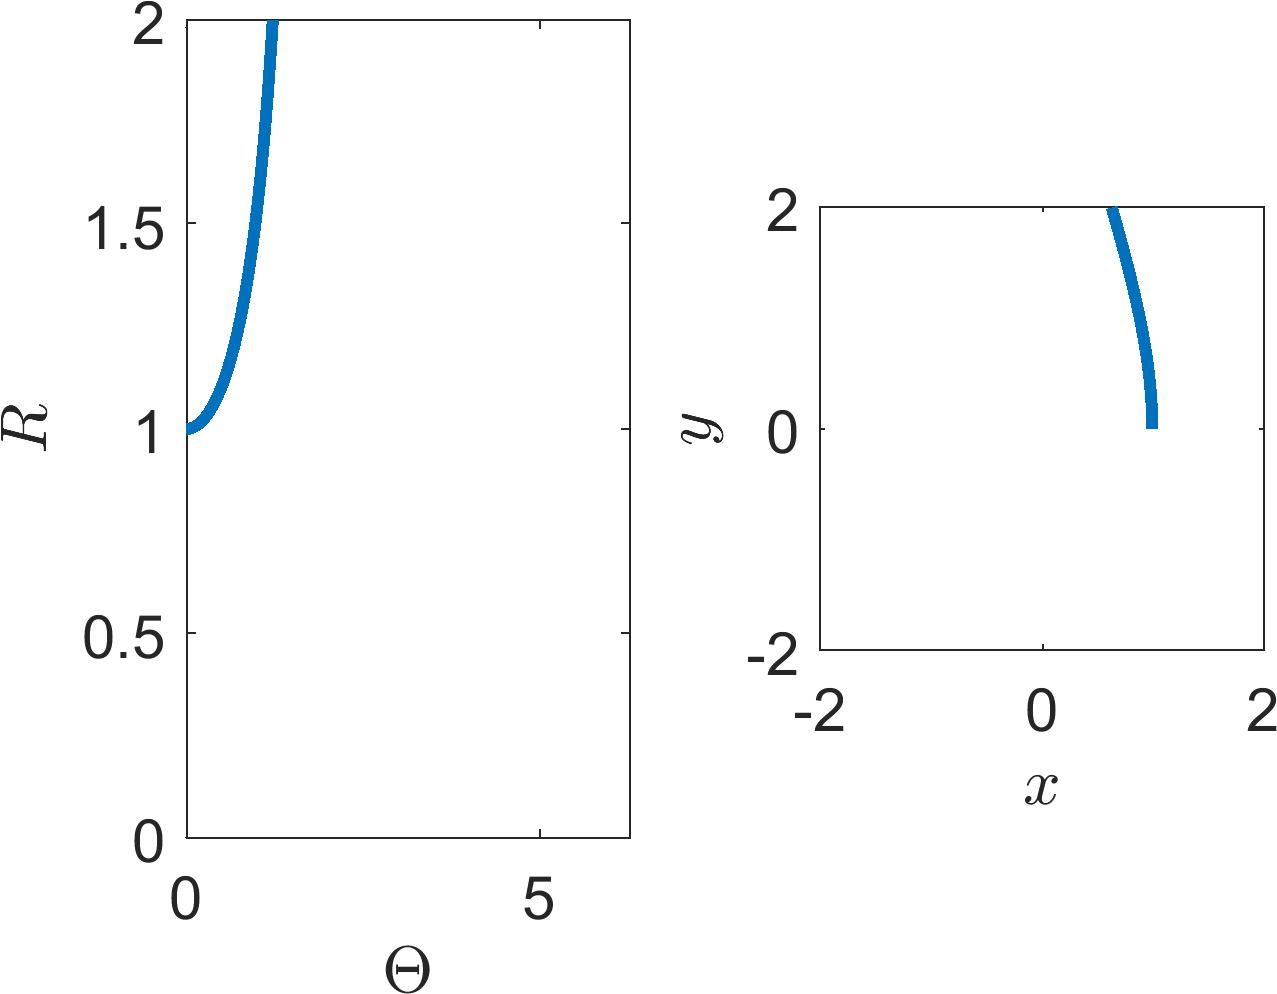
\includegraphics[width=\tttp]{../../Pictures/Orbit_a_025.png}}
\subfigure[]{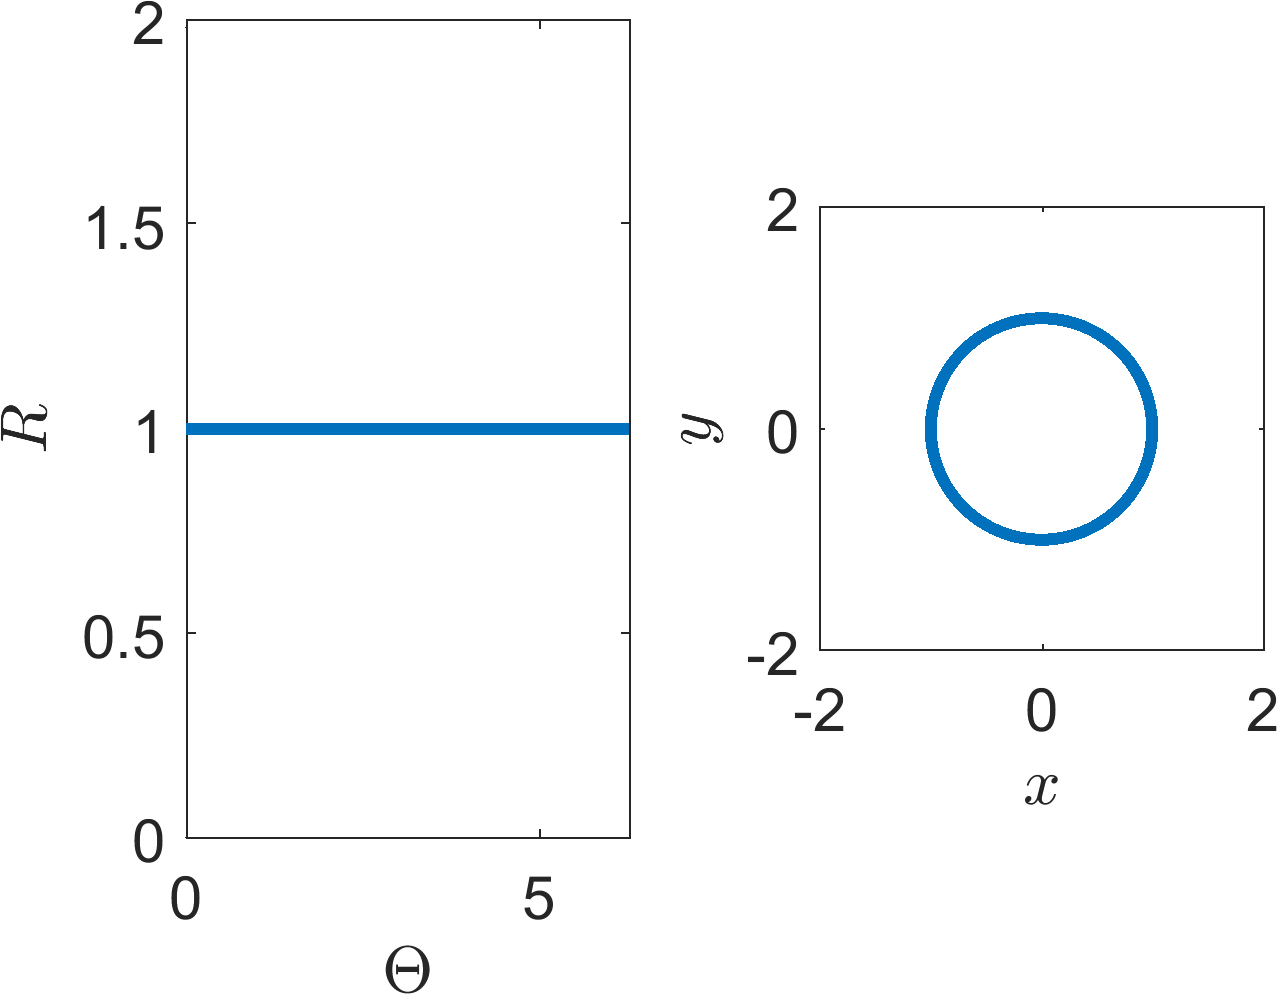
\includegraphics[width=\tttp]{../../Pictures/Orbit_a_1.png}}
\subfigure[]{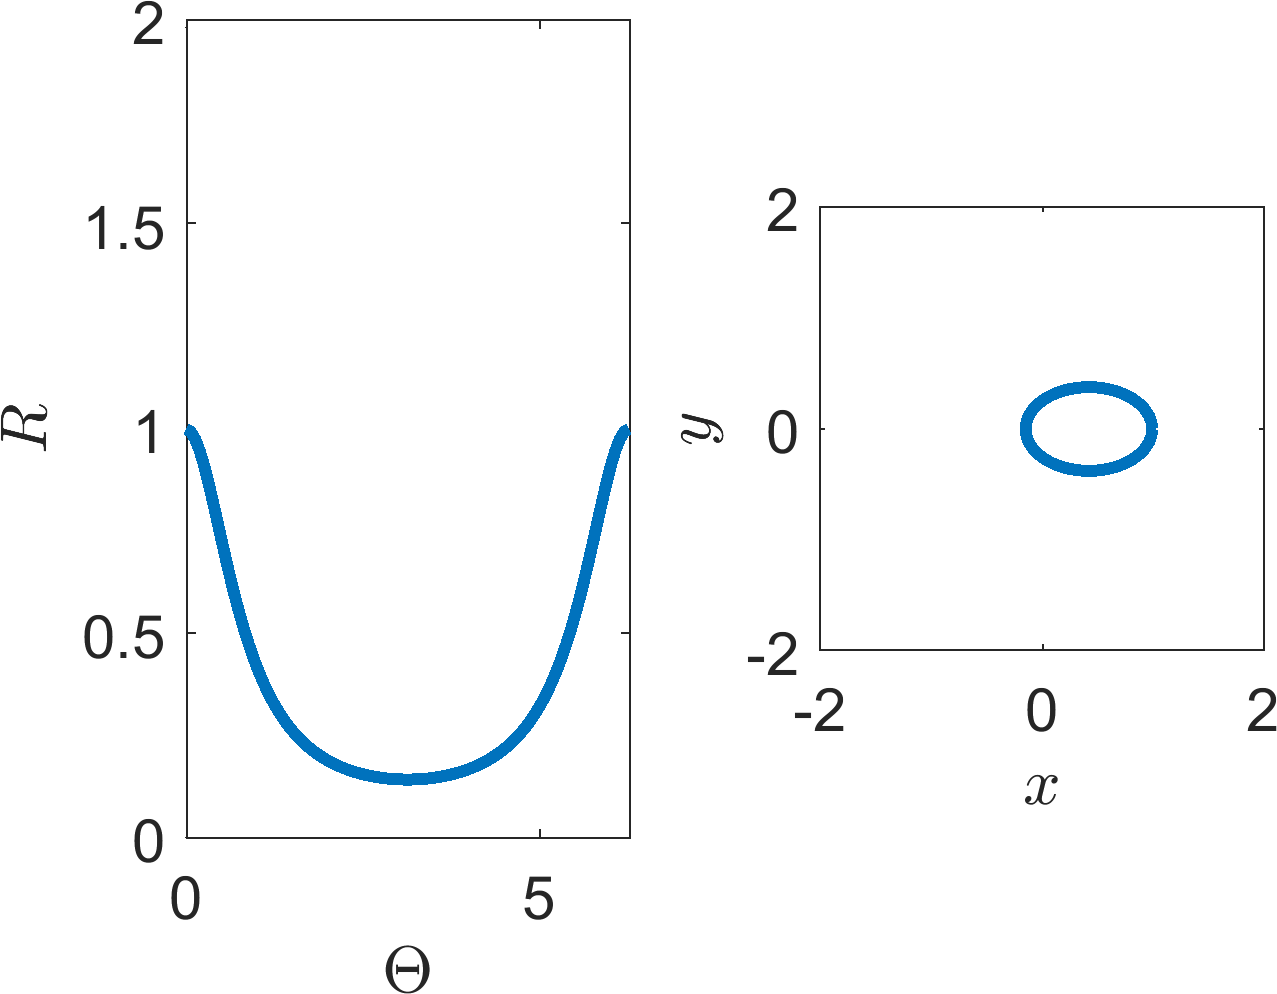
\includegraphics[width=\tttp]{../../Pictures/Orbit_a_4.png}}
\caption{\label{Orbits} Possible trajectories of \eqn{Radius}.}
\end{figure}
\begin{Answ}
\subsection{Answers}
\subsubsection{}
\begin{enumerate}[(a)]
\item  If $\alpha$ is really big then we get a very tight ellipse around the origin.
\item  If $\alpha=1$ we get a circle or radius 1.
\item  If $\alpha<1/2$ the function diverges to infinity as $\Theta$ increases. This means that the planet escapes the gravitational pull of the central planet.
\end{enumerate}
\subsubsection{}
If we make the identification $\alpha=Gm$ then we reproduce the planetary motion curve. Thus, for planets with very large mass we obtain highly elliptical orbits. For planets with a middling mass the orbits are circular. For planets with low mass the planets hardly effect one another and, thus, do not orbit.
\end{Answ}

\section{Law of Mass Action}
\begin{enumerate}
\item Write the following interaction equations as ODEs:
\begin{enumerate}
\item $3u\stackrel{r_3}{\rightarrow}2u\stackrel{r_2}{\rightarrow}u\stackrel{r_1}{\rightarrow}\slashed{0}$;
\item $2u+v\stackrel{r_1}{\rightarrow}v$, $2u\stackrel{r_2}{\rightarrow}\slashed{0}$, $2u+2v\stackrel{r_3}{\rightarrow}3u$, $\slashed{0}\stackrel{r_4}{\rightarrow}u+v$;
\item
\bb
u_1\mathrel{\mathop{\rightleftarrows}^{d}_{d}}u_2\mathrel{\mathop{\rightleftarrows}^{d}_{d}}u_3\mathrel{\mathop{\rightleftarrows}^{d}_{d}}\dots\mathrel{\mathop{\rightleftarrows}^{d}_{d}}u_{n-1}\mathrel{\mathop{\rightleftarrows}^{d}_{d}}u_n\nonumber.
\ee
\end{enumerate}

\item Write the following ODEs as interaction equations.
\begin{enumerate}
\item 
\bb
\dot{u}=r_1u\l 1- \frac{u}{r_2}\r\nonumber.
\ee
\item 
\begin{align}
&\dot{u}=-r_1uv-3r_2u^3,\nonumber\\
&\dot{v}=-r_1uv+r_3.\nonumber
\end{align}
\end{enumerate}
\end{enumerate}
\begin{Answ}
\subsection{Answers}
\subsubsection{}
\begin{enumerate}[(a)]
\item $\dot{u}=-r_1u-r_2u^2-r_3u^3$.
\item
\begin{align}
&\dot{u}=-2r_1u^2v-2r_2u^2+r_3u^2v^2+r_4,\nonumber\\
&\dot{v}=-2r_3u^2v^2+r_4.\nonumber
\end{align}
\item
\begin{align}
&\dot{u}_1=d(u_2-u_1),\nonumber\\
&\dot{u}_k=d(u_{k+1}-2u_1+u_{k-1}),\quad k=2,\dots,n-1,\nonumber\\
&\dot{u}_n=d(u_{n-1}-u_n).\nonumber
\end{align}
An interesting point to note about this last equation is that it is a finite element discretisation of the diffusion equation.
\end{enumerate}
\subsubsection{}
\begin{enumerate}[(a)]
\item $u\stackrel{r_1}{\rightarrow}2u$, $2u\stackrel{r_1/r_2}{\rightarrow}u$,
\item $u+v\stackrel{r_1}{\rightarrow}\slashed{0}$, $3u\stackrel{r_2}{\rightarrow}\slashed{0}$, $\slashed{0}\stackrel{r_3}{\rightarrow}v$. Alternatively, the first equation can be written as $u+v\stackrel{r_1}{\rightarrow}u$ and $u+v\stackrel{r_1}{\rightarrow}v$. Thus, the law of mass action transformation does not provide a unique mapping.
\end{enumerate}
%%
%%\item \textbf{Bacteria growth}
%%\dot{u}=v
%%\dot{v}=-uv
\end{Answ}
\section*{Exam revision}
\section{More two body problem}
From question \ref{Two body problem continued} we know that 
\bb
\ddot{R}-R\dot{\Theta}^2=-\frac{Gm}{R^2},\quad R^2\dot{\Theta}=C.
\ee
\begin{enumerate}
\item Use the second equation, above, to eliminate $\dot{\Theta}$ from the first equation.
\item Multiply the resulting equation by $\dot{R}$. Show that the equation can be rewritten in the following form
\bb
\frac{\rd}{\rd t}\l\frac{1}{2}\dot{R}^2+\frac{C^2}{2R^2}-\frac{Gm}{R}\r=0.
\ee
\item Integrate over time noting that initially $R(0)=R_0$ and $\dot{R}(0)=0$. Show that you can derive
\bb
\int^R_{R_0}\frac{\rd R}{\sqrt{C^2\l\frac{1}{R_0^2}-\frac{1}{R^2}\r+2Gm\l\frac{1}{R}-\frac{1}{R_0}\r}}=t.
\ee
\item Suppose a solution, $R(t)$, exists for all time, then we know that the term within the square root must be positive for all time. Letting $a=2Gm/C^2$ show that this means that if a solution exists then
\bb
(R_0-R)(R(R_0a-1)-R_0)>0.\label{Quad}
\ee
\item Consider the quadratic \eqn{Quad} and split the analysis into two cases.
\begin{enumerate}
\item Suppose $R_0a<1$, show that in this case if a solution, $R(t)$, exists for all time then $R>R_0$.
\item Suppose $R_0a>1$, show that in this case if a solution, $R(t)$, exists for all time then
\bb
\frac{R_0}{(R_0a-1)}<R<R_0, \quad \textrm{if $R_0a>2$} 
\ee
 and
\bb
R_0<R<\frac{R_0}{(R_0a-1)},\quad \textrm{if $1<R_0a<2$.}
\ee
\end{enumerate}
\end{enumerate}
\begin{Answ}
\subsection{Answers}
\subsubsection{}
Substitute $\dot{\Theta}=C/R^2$ into the first equation and simplify to get
\bb
\ddot{R}-\frac{C^2}{R^3}=-\frac{Gm}{R^2}.
\ee
\subsubsection{}
\begin{align}
&\dot{R}\ddot{R}-\frac{C^2}{R^3}\dot{R}=-\frac{Gm}{R^2}\dot{R},\nonumber\\
\implies&\frac{\rd}{\rd t}\l\frac{1}{2}\dot{R}^2+\frac{C^2}{2R^2}-\frac{Gm}{R}\r=0.
\end{align}

\subsubsection{}
\begin{align}
&\frac{1}{2}\dot{R}^2+\frac{C^2}{2R^2}-\frac{Gm}{R}-\frac{C^2}{2R_0^2}+\frac{Gm}{R_0}=0,\\
\implies &\dot{R}^2+C^2\l\frac{1}{R^2}-\frac{1}{R_0^2}\r+2Gm\l\frac{1}{R_0}-\frac{1}{R}\r=0,\\
\implies &\int^R_{R_0}\frac{\rd R}{\sqrt{C^2\l\frac{1}{R_0^2}-\frac{1}{R^2}\r+2Gm\l\frac{1}{R}-\frac{1}{R_0}\r}}=\int^t_0\rd t=t.
\end{align}
\subsubsection{}
A solution for $R(t)$ exists for all time if
\bb
C^2\l\frac{1}{R_0^2}-\frac{1}{R^2}\r+2Gm\l\frac{1}{R}-\frac{1}{R_0}\r>0.
\ee
Multiply through by $R_0^2R^2$ and divide through by $C^2$, all of which are positive.
\bb
\l R^2-R_0^2\r+aRR_0(R_0- R)=(R_0-R)\l aRR_0-R-R_0 \r=(R_0-R)\l R\l aR_0-1\r-R_0 \r>0.\label{ineq}
\ee
\subsubsection{}
If $aR_0<1$ the coefficient of the quadratic term is positive. The roots of the quadratic are $R_0>0$ and $R_0/(aR_0-1)<0$. Thus, for inequality \eqref{ineq} to be satisfied we need either $R>R_0$, as suggested in the question or $R<R_0/(aR_0-1)<0$, which is not possible since $R>0$.

If $aR_0>1$ the coefficient of the quadratic term is negative. The roots are $R_0$ and $R_0/(aR_0-1)$, which are both positive. For inequality \eqref{ineq} to be satisfied we $R$ needs to be between these two roots. However, the larger root depends on whether $(aR_0-1)$ is greater or less than one. If $(aR_0-1)>1$ then $R_0/(aR_0-1)<R_0$ and if $(aR_0-1)<1$ then $R_0<R_0/(aR_0-1)$, justifying the given ranges.
\end{Answ}
\section{More Law of Mass Action}
\begin{enumerate}
\item Write the following interaction equations as ODEs.
\begin{enumerate}
\item $u\stackrel{r_3/(1+u)}{\rightarrow}2u$.
\item $u+v\stackrel{r_1}{\rightarrow}v$, $u+v\stackrel{r_1}{\rightarrow}u$, $u+v\stackrel{r_1}{\rightarrow}\slashed{0}$.
\end{enumerate}

\item Write the following ODEs as interaction equations.
\begin{enumerate}
\item 
\bb
\dot{u}=1\nonumber.
\ee
\item 
\begin{align}
&\dot{u}=r_1uv/(1+v^2),\nonumber\\
&\dot{v}=-r_1uv/(1+v^2).\nonumber
\end{align}
\end{enumerate}
\end{enumerate}
\begin{Answ}
\subsection{Answers}
\subsubsection{}
\begin{enumerate}[(a)]
\item $\dot{u}=r_3u/(1+u)$.
\item $\dot{u}=-2uv=\dot{v}$.
\end{enumerate}
\subsubsection{}
\begin{enumerate}[(a)]
\item $\slashed{0}\stackrel{1}{\rightarrow}u$.
\item $u+v\stackrel{r_1/(1+v^2)}{\rightarrow}2u$.
\end{enumerate}
\end{Answ}
\end{document}